% !TeX spellcheck = en_US
% !BIB TS-program = biber
\documentclass[11pt]{article}

\usepackage{amssymb} % see: http://milde.users.sourceforge.net/LUCR/Math/mathpackages/amssymb-symbols.pdf
\usepackage{mathtools} % for extended mathematical symbols and more

% Page properties :
% See : https://tex.stackexchange.com/questions/36085/latex-without-pages
\usepackage{geometry}
\geometry{margin=25mm}

% Input file encoding :
\usepackage[utf8]{inputenc}

\usepackage[english]{babel}
\usepackage{lipsum}

\newcommand\BS{\char`\\}

\usepackage[
backend=biber,
style=numeric,
sorting=none
]{biblatex}
\usepackage{csquotes}
\addbibresource{Bibliography.bib}

% To color text :
% see : https://en.wikibooks.org/wiki/LaTeX/Colors
\usepackage[dvipsnames]{xcolor}


% To use images : 
\usepackage{graphicx} % use this
\graphicspath{ {./IMG/} } % path midifier for storing images
% to include a picture, type this ('name' is without path or extention) :
% \includegraphics[width=0.5\textwidth]{name}

\usepackage{dirtytalk}
\usepackage{parskip}

% How to use references :
\usepackage{hyperref} % use this
\hypersetup{
	colorlinks=true,    
	urlcolor=blue,
	citecolor=black
}

\usepackage{wasysym}

\usepackage{color}

\definecolor{mylightgray}{rgb}{0.95,0.95,0.95}

\usepackage[super]{nth}

% Regulates \tableofcontents max depth
\setcounter{tocdepth}{2}

\usepackage{array}
\newcolumntype{L}[1]{>{\raggedright\let\newline\\\arraybackslash\hspace{0pt}}m{#1}}
\newcolumntype{C}[1]{>{\centering\let\newline\\\arraybackslash\hspace{0pt}}m{#1}}
\newcolumntype{R}[1]{>{\raggedleft\let\newline\\\arraybackslash\hspace{0pt}}m{#1}}
\usepackage{xcolor,colortbl}
\newcolumntype{a}{>{\columncolor{mylightgray}}l}


\usepackage{listings}
\lstset{ 
	backgroundcolor=\color{mylightgray},   % choose the background color; you must add \usepackage{color} or \usepackage{xcolor}; should come as last argument
	basicstyle=\small,        % the size of the fonts that are used for the code
	breakatwhitespace=false,         % sets if automatic breaks should only happen at whitespace
	breaklines=true,                 % sets automatic line breaking
	captionpos=b,                    % sets the caption-position to bottom
	commentstyle=\color{mygreen},    % comment style
	deletekeywords={...},            % if you want to delete keywords from the given language
	escapeinside={\%*}{*)},          % if you want to add LaTeX within your code
	extendedchars=true,              % lets you use non-ASCII characters; for 8-bits encodings only, does not work with UTF-8
	firstnumber=1,                % start line enumeration with line 1000
	frame=single,	                   % adds a frame around the code
	keepspaces=true,                 % keeps spaces in text, useful for keeping indentation of code (possibly needs columns=flexible)
	keywordstyle=\color{blue},       % keyword style
	%language=Java,                 % the language of the code
	morekeywords={},            % if you want to add more keywords to the set
	numbers=none,                    % where to put the line-numbers; possible values are (none, left, right)
	numbersep=5pt,                   % how far the line-numbers are from the code
	numberstyle=\tiny\color{mygray}, % the style that is used for the line-numbers
	rulecolor=\color{black},         % if not set, the frame-color may be changed on line-breaks within not-black text (e.g. comments (green here))
	showspaces=false,                % show spaces everywhere adding particular underscores; it overrides 'showstringspaces'
	showstringspaces=false,          % underline spaces within strings only
	showtabs=false,                  % show tabs within strings adding particular underscores
	stepnumber=2,                    % the step between two line-numbers. If it's 1, each line will be numbered
	stringstyle=\color{mygreen},     % string literal style
	tabsize=2,	                   % sets default tabsize to 2 spaces
	title=\lstname                   % show the filename of files included with \lstinputlisting; also try caption instead of title
}

%% Define a HUGE : https://tex.stackexchange.com/questions/265/fonts-larger-than-huge
\usepackage{fix-cm}   
\makeatletter
\newcommand\HUGE{\@setfontsize\Huge{29}{35}}
\makeatother 

%% Adds padding to tables : https://tex.stackexchange.com/questions/64761/add-just-a-little-more-padding-to-my-table/381439
\usepackage{array}
\setlength\extrarowheight{2pt} % or whatever amount is appropriate

%opening
\title{\vspace{15mm}{\HUGE PoGER}\\
	A Bachelor's project}
\author{David Rodriguez Soares}
\date{}

% first page
\begin{document}
\maketitle

\vfill
%
\section*{Abstract}

Game development has evolved from an obscure activity only teams of people with specialized training could work on to an accessible art through the use of powerful tools and shared already-made code and assets, springing a healthy and successful independent game-making scene. Unfortunately, this is not the state of most fan-made game creation communities, in particular the one dedicated to the popular Pokémon franchise. It is plagued by a combination of issues, mainly the inadequacy of used tools, resulting in its apparent abandonment.

This paper presents PoGER, an software preservation and game engine recreation project aimed at proposing systemic solutions to these issues. I discuss the goals of this project, the reverse-engineering effort and its findings and design decisions taken. I also present a framework and tools for both porting old projects and facilitating future development, which could kickstart a new wave of enthusiasm in its field and hopefully give motivated developers an opportunity to create their own worlds and adventures.


\newpage

\begingroup
\hypersetup{linkcolor=black}
\tableofcontents
\endgroup
%
%\newpage




%This is intended to document my journey through my Bachelor's project. Some information may be omitted for brevity or because it is present in accompanying scripts.

%It can be decomposed \textbf{3 major steps} : \textit{inception}, \textit{research} and \textit{implementation}.

%\subsection{Related documents}
%
%This is but one in a collection of manuscripts, each with its scope (\textit{sorted older to newer}) :
%
%\begin{itemize}
%	
%	\item \textbf{Vision document} : A very early analysis about Pokemon Essentials, focused on identifying its issues and properties of a hypothetical software solution.
%	
%	\item \textbf{\textit{PoGER}} : Gives information on the project itself, including motivations and objectives.
%	
%	\item \textbf{RMXP doc} : Contains the results of my research about RPG Maker XP's implementation of game data (mostly \textit{Maps} and \textit{Events}), with the objective to extract them to an interpretable format.
%	
%	\item \textbf{Extraction} : Contain a practical guide on the extraction process for anyone trying to reproduce it.
%\end{itemize}


%\subsection{Notes}
%
%Here are some of the abbreviations you can encounter :
%\begin{itemize}
%	\item \textbf{RMXP} - RPG Maker XP
%	\item \textbf{RGSS} - Ruby Game Scripting System
%	\item \textbf{PE} - Pokemon Essentials
%	\item \textbf{PU} - Pokemon Uranium
%\end{itemize}
%
%Please note that the author is not a native English speaker.


\newpage
\section{Introduction}

Since its creation by japanese game designer  Satoshi Tajiri in 1995 \cite{PkmnCreator,SatoshiBook}, the Pokémon franchise (also known as \textit{Pocket Monsters} in Japan) had a significant impact on culture around the world \cite{PkmnPop,PkmnEffect} and on its own genre (the JRPG, for Japanese Role-Playing video Game) \cite{PkmnRPG}.

The Pokémon games, originally launched on the Nintendo Game Boy handheld, experienced immediate and global success, selling over 46 (or 31 if not counting \textit{Pokémon Yellow}) million units on its first generation \cite{PkmnSales} and more than 368 million copies sold overall \cite{PkmnFigures}.

\begin{figure}[!h]
	\centering
	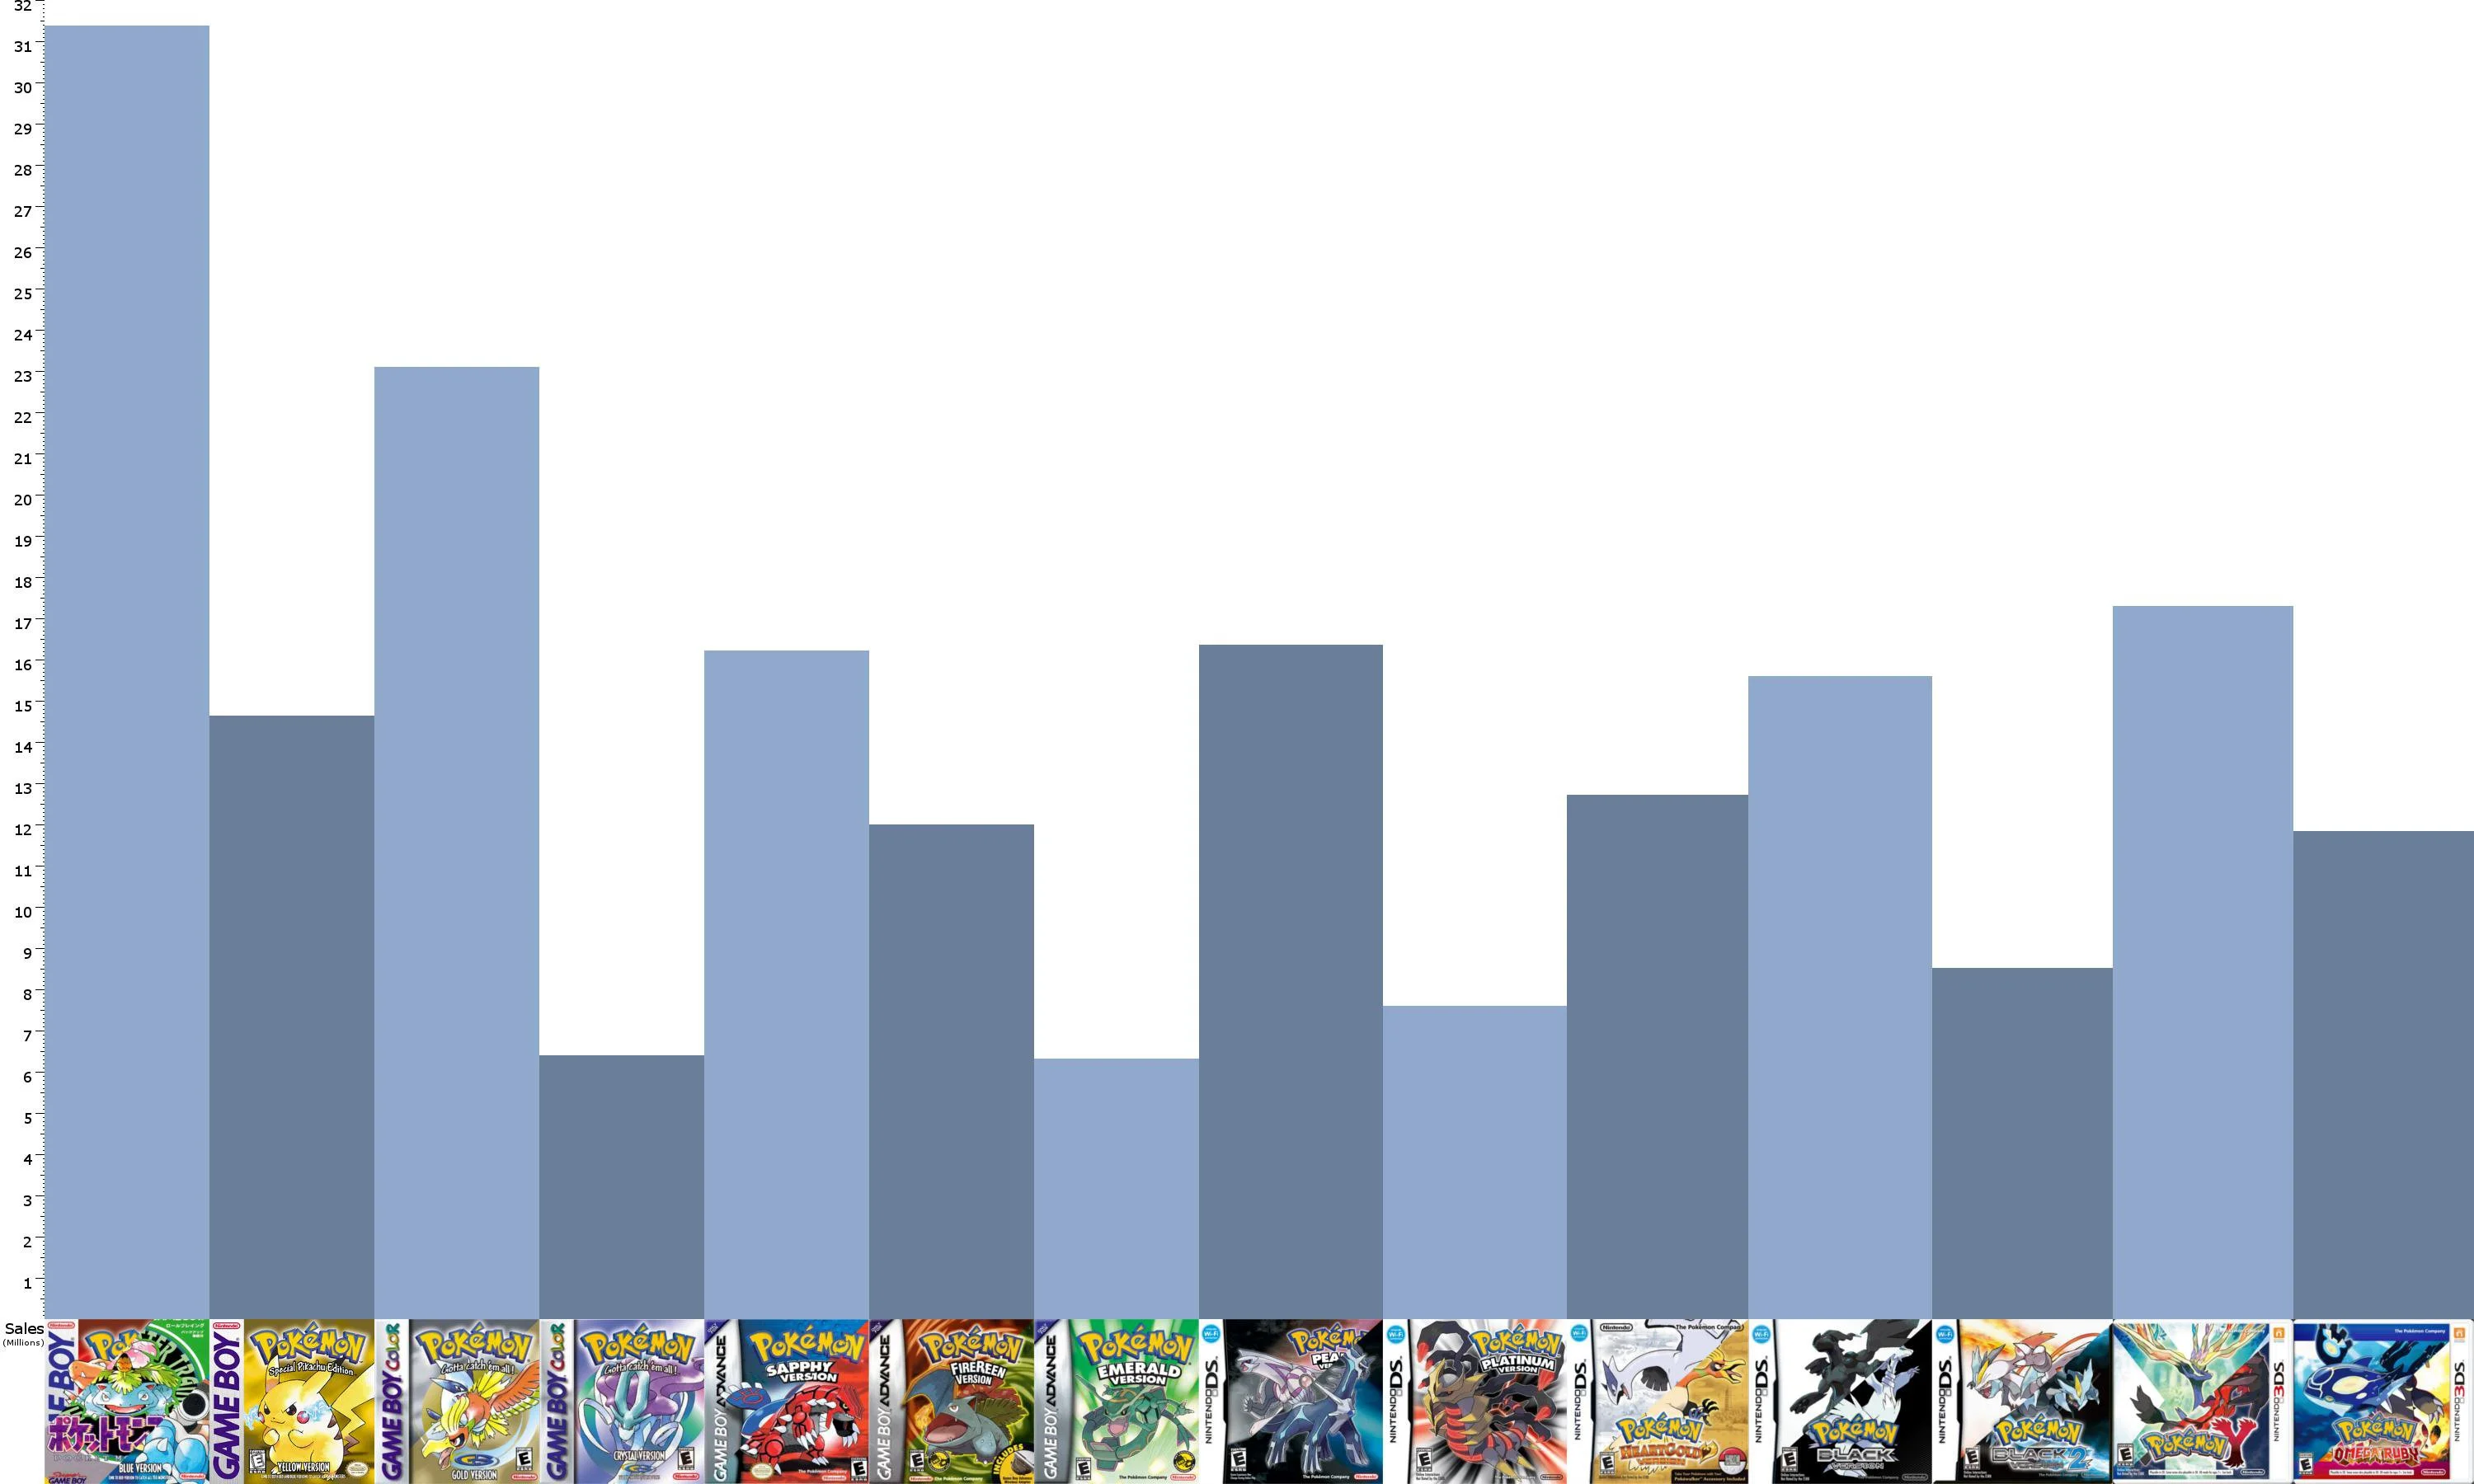
\includegraphics[width=\textwidth]{Pokemon_sales_gen}
	\caption{Unit sales of Pokémon mainline games, in millions \cite{PkmnSales,PkmnSalesIll} }
\end{figure}

Since then, it influenced generations of people who created art \cite{PkmnArt}, named animals and proteins \cite{Pikachurin,Etymology}, wrote novels \cite{Novel}, did scientific research, etc. Simply search for \texttt{Pokémon} on an academic search engine like \texttt{Google Scholar} and you would be surprised of the amount of results and the diversity of represented fields !

With such a motivating and long-running game franchise, it was inevitable some fans would look into the possibility of making their own addition to the series.

\subsection{The state of Pokémon fan-made games}

As the name suggest, these games are created by fans of the franchise and are based on its core concepts and gameplay mechanics \cite{PkmnFangames}. Over the last two decades, many game projects saw a release on the Internet and even a few can be found in physical media form \cite{PkmnUV,PkmnCartridge} !

But what does that development scene looks like ? What I discovered was a clustered universe of fan-made games. There are 3 main categories : 

\textbf{ROM hacks} \ Build upon the code and assets of commercial products, typically GameBoy games \cite{PkmnFangames}, they can be played on common emulators (and on original hardware \cite{Homebrew}), therefore available for most platforms. Unfortunately, programming for them is very technical, with limited functionality and questionable legality \cite{PkmnRH}.

\textbf{Games made with RPG Maker XP} \ Build on top of the \textit{Pokemon Essentials} project \cite{PkmnFangames,Essentials}, they are easier to program for and have less limitations than ROM hacks.

\textbf{Original games} \  These are original software, typically built for Windows or the web. Thanks to that, they can have great performance and novel game mechanics (eg. MMORPG style), but remain typically closed-source, and only a few projects exist \cite{PkmnPlanet, PkmnLegends, PkmnFanGameList}.


\subsection{Problems}

% Problématique

A lot of people tried to make their own games by love for the franchise, but from my early research into Pokémon fan-made games, a few common issues can be identified.

Except for ROM hacks and the occasional web-based game, which run on emulators and web browsers respectively, software is \textbf{platform-specific} (typically made for the Windows operating system). This is not optimal, because it restricts the amount of devices they can be run on, thus their market. Combined with the fact that they are almost universally \textbf{closed-source}, it becomes an issue of \textbf{software conservation}.

Another common issue is the \textbf{high amount of technical knowledge} that anyone willing to work on them needs, even with tools like RPG Maker XP.

Due to the \textbf{legality challenges} and the \textbf{personal nature} of fan-games, but also the \textbf{lack of collaborative code source management tools} (like \textit{git}), they are typically a \textbf{single-developer endeavor}. 

The combination of previously mentioned issues is, in my opinion, a perfect storm that explains the lack of quality fan-made games in a time independent game development is on the rise : It kills most attempts before they are release-worthy and keeps the rest from ever becoming polished and rid of bugs as commercial games. 

This happens because their developer finds no more time to invest or lose interest in them, and picking them up once that happened can be incredibly difficult, or even impossible.

This motivated me to find a solution that would addresses these issues, but I knew it was unrealistic to do so for every category of games.


\subsection{Focusing on Pokemon Essentials}

RPG Maker XP is an popular but aging RPG engine that offers convenient tools that allows anyone to make their own role-playing video game \cite{RMXP}.

Unfortunately, programming for it is technical and it's only compatible with Windows (even running games on compatibility layers such as Wine on GNU/Linux isn't always functional). Also, performance is typically poor due to its aging engine \cite{PoorPerf}.

\textbf{Pokemon Essential} is a project that aims at offering an implementation of the Pokemon game engine that runs on RPG Maker XP. Few projects using it were completed \cite{PkmnFangames}.

Even with the facilities introduced, programming for RPG Maker XP/Pokemon Essentials remains complex, and is typically done in very small teams of amateurs, not using collaborative source code management tools like \textit{git}. This results in ambitious project requiring years before they can be released and are hard to maintain (see \texttt{Pokémon Uranium} for a case study).

I believe this is the reason most projects never see a release, and the ones that do are buggy.


\subsection{Defining the project}

%I started by identifying shortcomings of the studied software, then moved on to coming up with solutions.

The problem can be stated more simply : RPG Maker XP/Pokemon Essentials isn't adapted to creating a game in a modern way, and suffers from its age and design decisions, to the point it's basically abandoned and deprecated. Also, there doesn't seem to be a superior alternative tool for the purpose of creating a Pokemon game. It's clear to me that I should not try to build upon it, but rather bring it up somehow.

I won't detail every design decision here, but each one was made toward the goal of addressing the identified shortcomings of the studied software. Please read the \textit{vision document} for more information.

The solution I came up with : implementing a similar engine that would be decoupled from RPG Maker XP  and would run games as programs written in an interpreted domain-specific language I would create. A complementary piece of software would automate the port of games written for the original Pokemon Essentials engine, therefore making it more relevant than an alternative without any retro-compatibility path.

There is a name for this approach : \href{https://en.wikipedia.org/wiki/Game_engine_recreation}{game engine recreation}.  That's where the name for this project comes from, \textbf{PoGER} (\textit{\textbf{Po}kémon Essentials \textbf{G}ame \textbf{E}ngine \textbf{R}ecreation}).

\textbf{Requirements} : A solution would be an implementation of Pokémon Essentials that is : 
\begin{itemize}
	\item performant
	\item available (multi-platform)
	\item straightforward and simpler to develop for
	\item has online capabilities
	\item has engine code separate from game code
	\item provides documentation, sets standards
	\item fundamentally open-source to allow contributors to maintain projects.
	\item has a way to port games from the original Pokémon Essentials
\end{itemize}

\vspace{4mm}

\subsection{Outline}

This report is divided in six sections, including this introduction.

\begin{itemize}
	\item Section 2 briefly explores the modern preoccupation of software perservation and discusses the application of its principles to the current project.
	
	\item Section 3 gives a detailed summary of identified software and projects of interest.
	
	\item Section 4 looks into the feasibility of asset and feature extraction from an existing Pokémon Essentials project. Then, it presents the implementation results of the extraction process and details the steps involved in a practical guide fashion.
	
	\item Section 5 presents the reverse-engineering results for a particularly complex category of extracted assets : Events. This is followed by a discussion on the necessity of a new representation for them and the design decisions behind the proposed domain-specific language. A formal definition is given, with examples and a Python implementation.
	
	\item Section 6 presents the early work on \texttt{PEN}, an interpreter that can run events. This would be the basis for an interpreter capable of running a full game. A portion is dedicated to PBS files and information that can be imported from them.
	
	\item Section 7 covers the reverse-engineering efforts aimed at interpreting RPG Maker XP's proprietary map and map asset format. Then, it presents a proof of concept implementation in Python.
	
	\item Section 8 explores the future of the project, the path towards an actual implementation of an interpreter capable of executing games, providing directions for future work.
	
	\item Section 9 closes this report with a summary and a critique of its contributions.
\end{itemize}







\newpage

\section{About software preservation}

\subsection{Maintaining the ability to run software}

A modern preoccupation is the preservation of aging hardware and software, because as time passes, functional ancient hardware becomes increasingly scarce, and with it the means to run software made for it.

The problem of maintaining the possibility to run software despite the loss of access to its original platform pushed the development of \textbf{virtualization and emulation technologies}.

* Mendel Rosenblum: The Reincarnation of Virtual Machines. ACM Queue 2(5): 34-40 (2004)

* Bowen Alpern et al.: The Jikes Research Virtual Machine project: Building an open-source research community. IBM Systems Journal. 44(2): 399-418 (2005)

\subsection{Preserving source code}

Another related preoccupation is the long-term preservation of source code.


\section{Research subjects}

In order to define the scope of this project, I had to become familiar with the games and tools used to make them. In this section, I detail relevant information on RPG Maker XP/Pokémon Essentials

\subsection{RPG Maker XP}


According to its \href{https://en.wikipedia.org/wiki/RPG_Maker#RPG_Maker_series_timeline}{Wikipedia article} and its \href{https://www.rpgmakerweb.com/products/programs/rpg-maker-xp}{official website}, RPG Maker XP was developped by Enterbrain and released on July of 2004 for Microsoft Windows. 

It allows its users to create their own role-playing game with powerful dedicated tools and its engine is based on the Ruby programming language, making complex behavior possible through the use of \textit{scripts}.


This is only one instance among the long line of RPG Maker releases, some of which were released on other platforms, including consoles. Probably due to its early popularity, new projects continued to use this version way after it was superseded by newer ones.



\subsubsection{Ruby Game Scripting System}

\href{https://rmvxace.fandom.com/wiki/RGSS}{From this article} : 

\say{RGSS stands for Ruby Game Scripting System, a library that has been used in RPG Maker engines since RPG Maker XP.  It's a Ruby library, and as such, all scripting is done in the Ruby language.
	
In all of its incarnations, RGSS has included objects and methods with which to handle graphics, audio, and data, including basic data structures for the RPG Maker engine.

The original version, RGSS, [...] was based on Ruby 1.81.}

RGSS's latest version, RGSS3, was introduced with RPG Maker VX Ace in 2011-2012.






\subsection{The Pokemon Essentials project}


According to its \href{https://essentialsdocs.fandom.com/wiki/Essentials_Docs_Wiki}{wiki fandom page} and \href{https://pokemon-fan-game.fandom.com/wiki/Pok\%C3\%A9mon_Essentials}{another wiki article}, Pokemon Essentials is \say{a collection of gameplay-altering original code designed for use in an RPG Maker XP game}.

This means that it's a \textbf{RMXP project}, made to be the basis for a game. It was forked from Flameguru's Pokémon Starter Kit and developed by Peter O. (2007-2010) and Maruno (2011-today).

This project is up-to-date with the \nth{5} generation of the mainline Pokemon games and is the basis of a fair proportion of Pokemon fan-made games. It was last updated in October of 2017, when it was hit by DMCA takedown notice.


\subsubsection{Digging for information on Pokemon Essentials}

Users have been able to produce content-adding patches, like support for newer generation creatures, items and abilities.

There is \href{https://www.reddit.com/r/PokemonRMXP/comments/ckeaov/pok\%C3\%A9mon\_essentials\_v18\_progress\_report/}{a v18 in the works} (release date unclear). \href{https://www.reddit.com/r/PokemonRMXP/comments/hb6i6m/should\_i\_wait\_for\_essentials\_v18/}{On Reddit}, Maruno stated "hopefully it won't be long now" in June 2020.

It is notably hosted on  \href{https://archive.org/details/PokmonEssentialsV17.220171015}{archive.org} but I downloaded it from \href{https://mega.nz/file/HPQDCIaY#Ie9LcVXeFgiLElIFmyx9uv6lwuyw8P-1REEoqnW7USs}{this source} because it has a Wikia dump and later file modification timestamps.





\subsection{The Pokemon Uranium project}


According to its \href{https://en.wikipedia.org/wiki/Pok\%C3\%A9mon_Uranium}{Wikipedia page}, its \href{http://pokemonuranium.org/}{official website} and its \href{https://pokemon-uranium.fandom.com/wiki/Main_Page}{Fan-made Wiki website}, Pokemon Uranium is a fan-made game based on Pokemon Essentials (version used is unclear) and has unique region, creatures, assets, plot and quests. It is often cited as one of the best Pokémon fan-made game \cite{PkmnBestFG, PkmnBestFG2}.
It was developped by a small team for about 9 years and released in August 2016.
\begin{itemize}
	\item Game designer and developer : JV12345 (aka. $\sim$JV$\sim$)
	\item Game developer and creative director : Nageki (aka. Involuntary Twitch)
\end{itemize}
They were hit by DMCA takedown notices shortly after release and stopped development in September 2016 \cite{PUtakedown}.


\subsubsection{Digging for information on Pokemon Uranium}

The game was mostly complete when released, but its website and following game updates are community efforts. Fans were able to add elements to push it farther towards completion but there still are some hanging threads, particularly in the post game (after the main plot is over) \cite{PUsidequests}.

Fans have been able to patch bugs and update the game for some time. I suppose there is a small group of people with access to the project's source code and files that have been maintaining it and its online services. Despite efforts to patch it, the game has a \href{https://pokemon-uranium.fandom.com/wiki/Bugs_and_Errors}{long list} of unresolved bugs and game breaking/crashing situations.
	
I wasn't able to identify the used versions of RPG Maker XP or Pokemon Essentials, but I determined this wouldn't significantly impact on working on it.
	
GitHub user \textit{acedogblast} launched a \href{https://github.com/acedogblast/Project-Uranium-Godot}{re-implementation project} on the Godot game engine in early 2019. As of writing, he states that :
	\say{Only a limited portion of the game is playable currently.}
	
Download links are hosted \href{https://www.reddit.com/r/pokemonuranium/comments/a0cw0i/download_links/}{on Reddit}. Current version is \verb|1.2.4| and was released on October \nth{29} 2018.



\newpage 
\section{Extracting existing game assets}

This section covers the complementary pieces of software that assist and automate the port of Pokemon Essentials. Games based on Pokemon Essentials should be able to be ported through the same process, with perhaps a few tweaks.

The information presented here was obtained through the official RPG Maker XP built-in documentation, user content found on the internet (forum posts, videos) and the author's reverse-engineering work.

Unless otherwise specified, the following findings pertains to the \texttt{Pokémon Essentials v17.2} project files and may not always apply to derivatives. 


\subsection{Technical findings}

\subsubsection{Structure}

Pokemon Essentials and its derivatives can be downloaded and their root directory explored without any specialized tool but perhaps an archive extractor utility. They all share this project structure :

\begin{tabular}{|r L{.1\linewidth}|L{.8\linewidth}|}
	\hline
	$\circ$ & Root & Contains compiled game files and libraries, plus a few useful programs, some probably made by Pokemon Essentials developers. \\
	\hline
	\rotatebox[origin=c]{180}{$\Lsh$} & Audio & Contains the musical assets of the game, typically MIDI and OGG files. \\
	\hline
	\rotatebox[origin=c]{180}{$\Lsh$} & (Data) & Contains the logic of the game and most of its data.  \\
	\hline
	\rotatebox[origin=c]{180}{$\Lsh$} & Fonts & Contain fonts used for displaying text. \\
	\hline
	\rotatebox[origin=c]{180}{$\Lsh$} & Graphics & Contains the graphical assets of the game, typically tile sets, in a well organized folder structure. \\
	\hline
	\rotatebox[origin=c]{180}{$\Lsh$} & (\textit{PBS}) & Contains human-readable data to be compiled, like items, species, types, dialogue (and translations), etc. \\
	\hline
\end{tabular}

Note that in certain circumstances, directories shown between parenthesis may be omitted, because they exist in a compiled form. This is typical for game releases as it's a more efficient format for execution. This will be expanded upon thereafter.


\subsubsection{Data representation}

The data that constitutes a PE project is diverse :

\begin{tabular}{|L{.1\textwidth}|L{.52\textwidth}|L{.3\textwidth}|}
	\hline
	\rowcolor{mylightgray}
	\textbf{Category} & \textbf{Description} & \textbf{Storage} \\
	\hline
	Scripts & Logic of the game, classes, ect & \verb|Scripts.rxdata| file \\
	\hline
	Objects & Files containing sets of class instances, grouped per file & \verb|dat| and \verb|rxdata| files \\
	\hline
	Maps & Contain map representation (incl. events), one per file & \verb|MapXXX.rxdata| \\
	\hline
	Dialogue & Contain dialogue & TODO \\
	\hline
\end{tabular}


\subsection{Research}

In order to decouple PE from its original code base and RGSS, it became obvious that all useful data had to be extracted from the project.

Since \verb|Audio|, \verb|Graphics| and \verb|Fonts| directories contain already-accessible data, they didn't require any extraction efforts.

See section \textit{Data representation} for categories of data that were identified to need extraction.


\subsection{Scripts}

Findings :
\begin{itemize}
	\item \verb|Scripts.rxdata| is the second largest compiled file of the project, and contains over 120k lines of code.
	
	\item The script is unique : it is divided in named sections (that appear in RMXP's editor on the left hand side) that allow to manage its colossal line count.
	
	\item Like other compiled files, its content are almost impossible to read outside of RMXP.
\end{itemize}

I spent quite a lot of time working on a python script able to decrypt \verb|rxdata| files, and \verb|Scripts.rxdata| in particular, but didn't have much success, so I tried looking elsewhere.

\textbf{Trying something else} : After some more digging, I found a functional utility that was created for the purpose of editing/extracting the scripts from this file : Gemini Editor.

Here are links to \href{https://forum.chaos-project.com/index.php/topic,10420.0.html}{a forum post about it} and \href{https://github.com/terabin/Gemini}{a github repository}.

With it, I was able to extract Pokemon Essentials scripts (see '\verb|PE_scripts|' directory).

It proved invaluable to be able to explore/search the whole script base using a more powerful code editor, saving lots of time from my attempts to create my own scripts to export data.

Note that extracting scripts isn't really useful : the objective is to get away from the RMXP-tied original codebase. It's only useful for the purpose of understanding how RMXP/RGSS/PE work and how features are implemented.


\subsection{Maps and Events}

Maps are essential to games made with RMXP, and a huge portion of the interface is dedicated to them. They contain textures that build the world and events that add elements of behavior to them.

I documented all I could find on maps the events they contain and more in \verb|RMPX_doc|.

What I found :
\begin{itemize}
	\item Trying to extract everything from compiled files would require a lot of effort.
	
	\item Creating scripts in RMXP that extract data is way easier.
	
	\item A solid understanding of the Ruby language and classes involved is mandatory.
	
	\item Class declarations can be found in the code and/or in the official documentation with a bit of digging.
\end{itemize}

\vspace{4mm}
Here is a diagram for classes involved in Map/Event/Tileset data extraction.
\begin{figure}[!h]
	\centering
	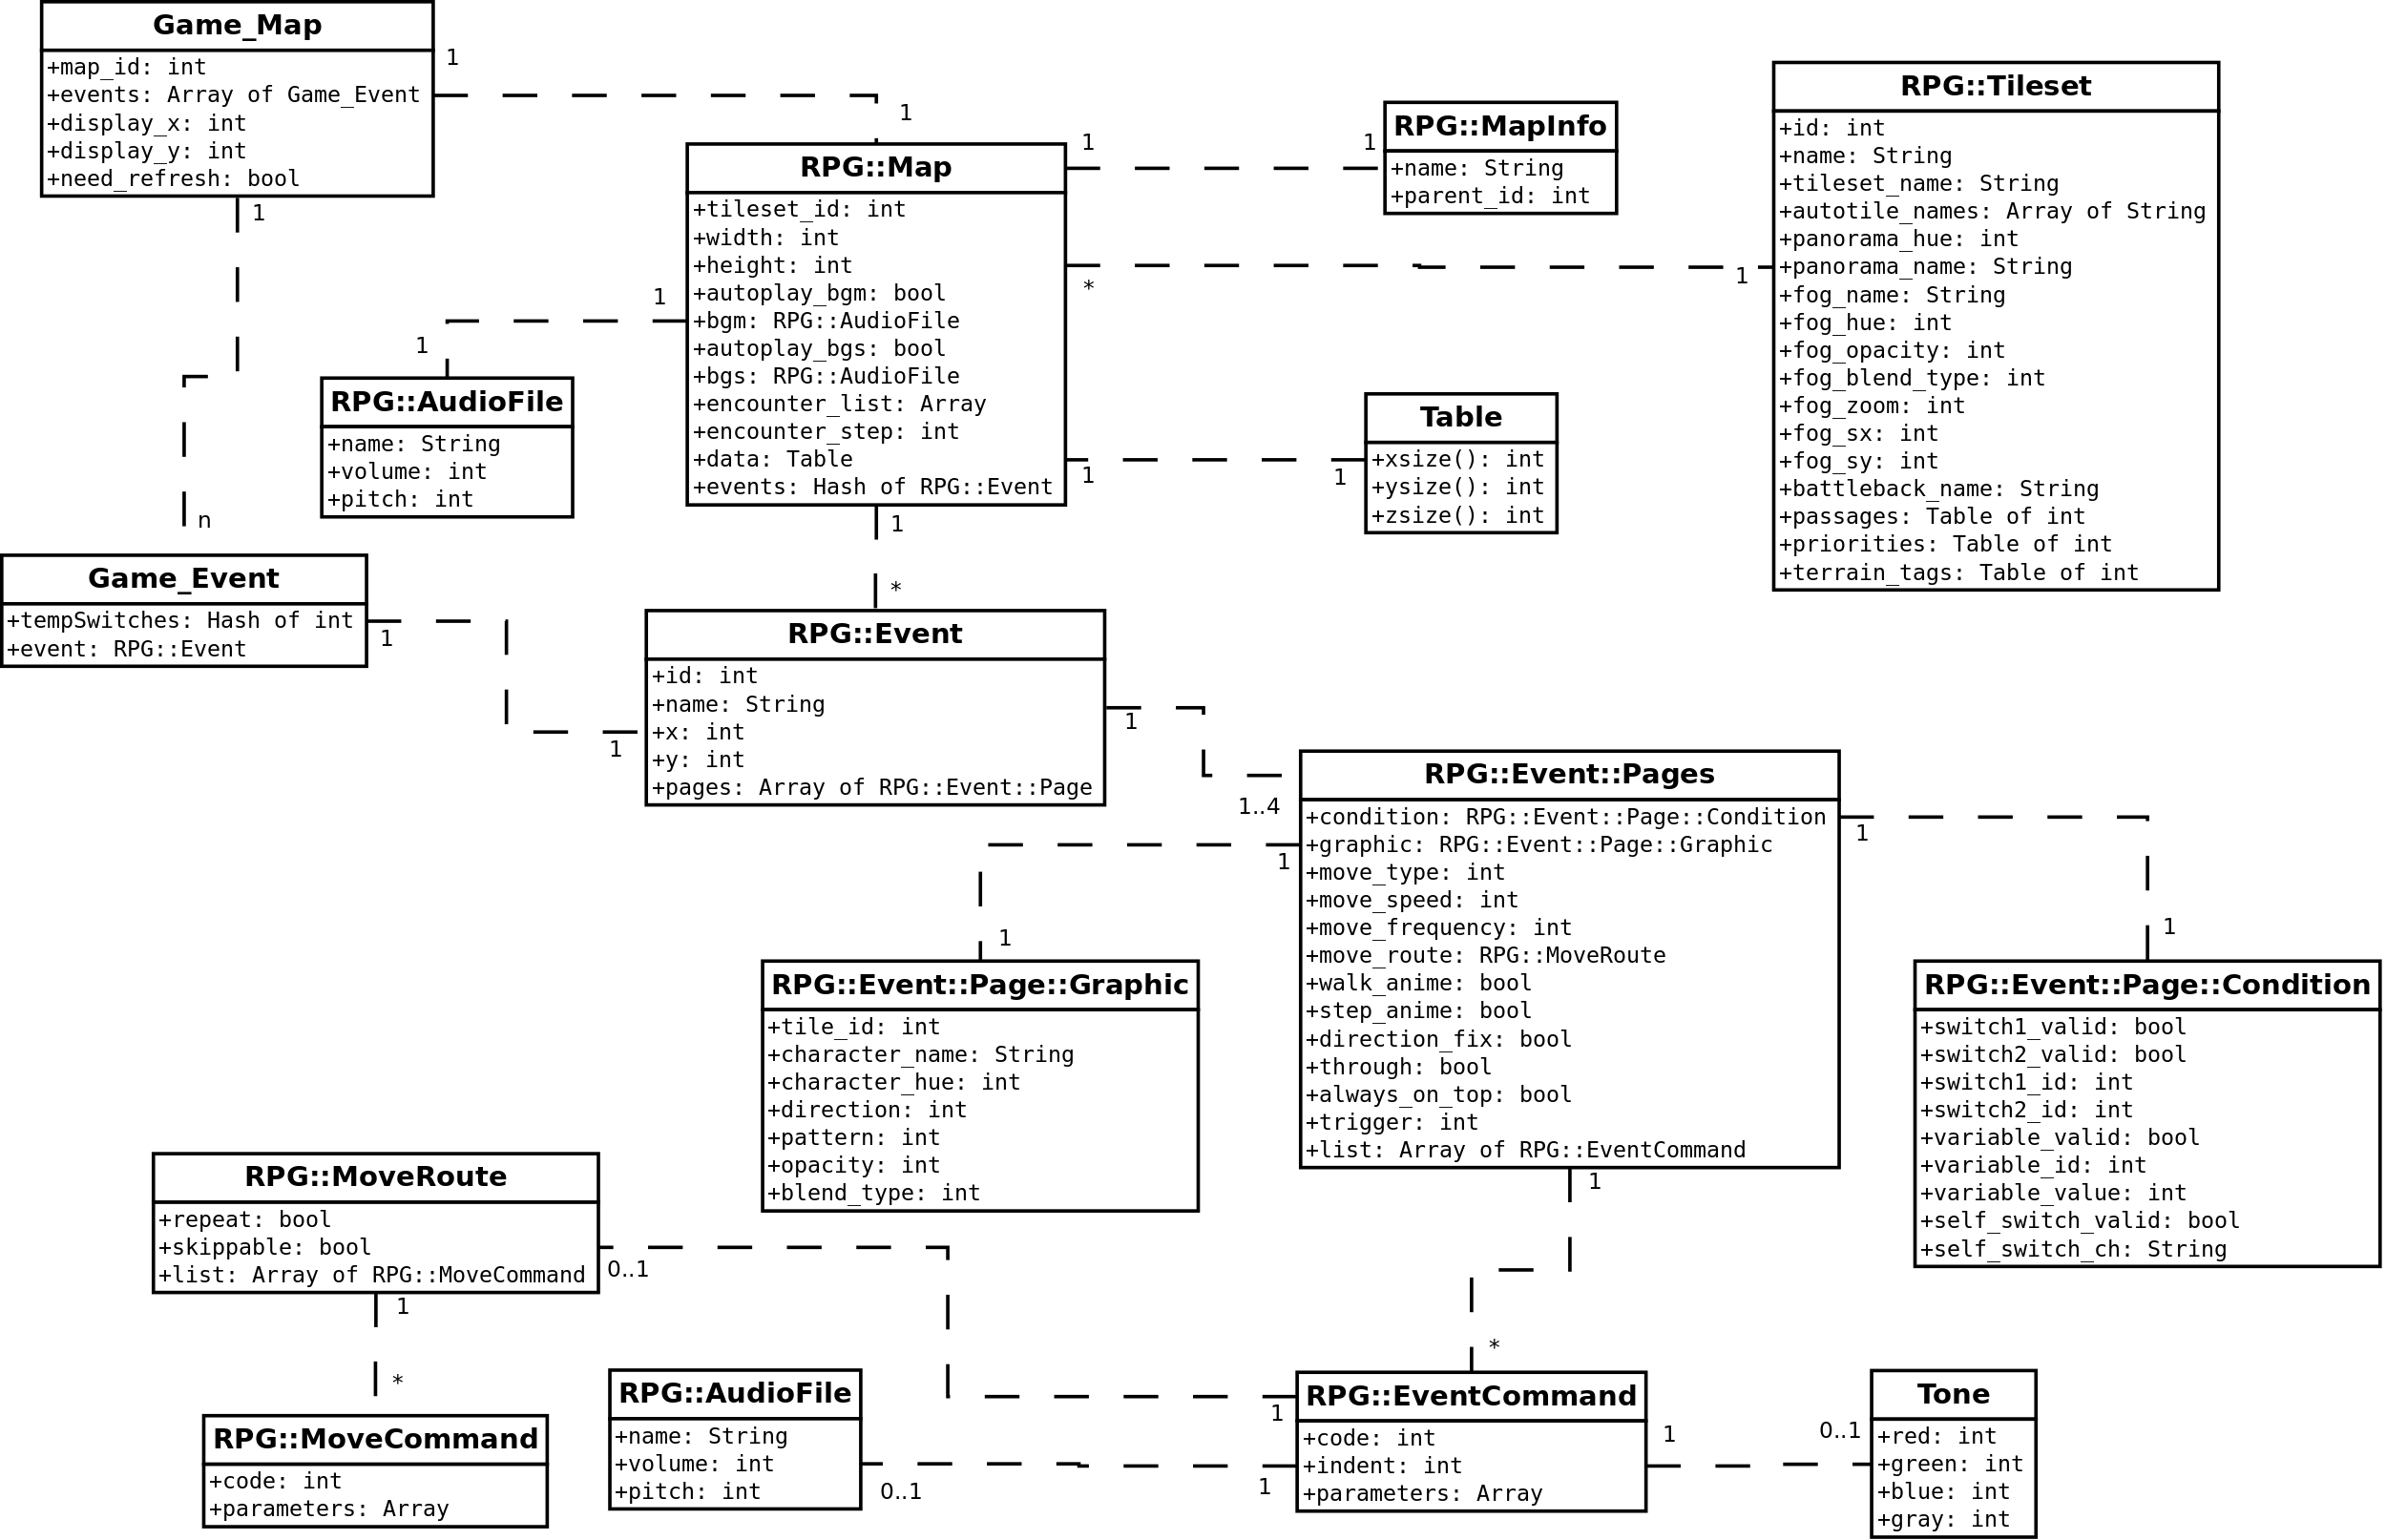
\includegraphics[width=\linewidth]{RMXP_full}
	\caption{Simplified class map representation for Map/Event}
	
\end{figure}


\textit{Semantic/Syntax} : Linked classes (with arity) display an \textbf{associative relationship}.

\textit{Note} : There is no inheritance relationship between any two classes represented. Arities are logically deduced and may not be exact depending in proprietary implementation details. Class \verb|RPG::AudioFile| was duplicated for ease of association routing.


\subsubsection{Dialogue}

English dialogue is hard-coded in events, therefore in order to propose alternative languages some trickery is needed.

More research is needed here.


\subsection{Automated extraction process}

Unfortunately, the first steps require the use of RPG Maker XP (version 1.02 tested, other may work also), and therefore Microsoft Windows (XP-10).

It may be possible to run RPG Maker XP on other operating systems using compatibility layers (such as Wine for GNU/Linux), but I didn't try it.

\subsubsection{Opening a project with RPG Maker XP}

First things first, a copy of the project to extract is needed. It should have the same structure as described in \verb|section 1.2.1|. If so, it should be possible to open it and run it using RPG Maker XP.

Read more about obtaining a copy in \verb|PoGER|.

The following information was obtained through a trial-and-error process when trying to open the Pokemon Essentials and a derivative game (Pokemon Uranium) in RPG Maker XP and run them in order to extract data from them. As such, they may contain erroneous statements or not apply/work for someone else trying to replicate the same process.

\begin{itemize}
	\item You need the following files in the root directory :
	
	\begin{itemize}
		\item \verb|Game.exe| : The executable that launches the game.
		\item \verb|Game.ini| : A configuration file. If the \verb|*.ini| in the project has an other name, \textit{rename a copy} and \textbf{leave the original untouched}, because it seems RMXP needs a \verb|Game.ini| file and game can specify an other name (hard coded in scripts)
		\item \verb|Game.rxproj| : Entry point for RMXP.
		\item \verb|RGSS102E.dll| : Contain RGSS dynamic libraries, probably necessary tu run the executable correctly.
	\end{itemize}
	
	Renaming files may be needed for some project files.
	
	\item For projects with \textit{compressed data} (no \verb|Data| directory but there is one \verb|*.rgssad| file at root), you need to use an extraction utility.
	
	I used \href{https://gitlab.com/rgss/rgsstool}{RGSS Tool} :
	
	\begin{lstlisting}
	python rgsstool.py -x -d "path\for\output\files" "path\of\rgssad\file"\end{lstlisting}
	\vspace{-8mm}
	
	This worked with Python 3.x, google search it if you're not sure if you have a recent version of Python and how to launch it on your computer.
	
	Exemple for Pokemon Uranium when command line is at root :
	
	\begin{lstlisting}
	python rgsstool.py -x -d . Uranium.rgssad\end{lstlisting}
	\vspace{-6mm}
	
	\item For projects missing the \verb|*.rxproj| file, simply create a new empty file and write the following: 
	
	\fbox{\ttfamily RPGXP 1.02}
	
	Save it with UTF-8 encoding and no "new line" character.
	
	\item Save files should be located in \verb|C:\Users\<user_name>\Saved Games\<name_of_the_game>\|
	
	\item Tip : When running the project from RPG Maker XP, some files in the \verb|Data| directory may be recompiled, which can cause errors. Keep a copy of the content of this directory in case you need to restore its content (you can exclude the \verb|Scripts.rxdata| if you're editing the scripts, so you don't lose progress on this file).
\end{itemize}


\subsubsection{RMXP script}

The first step uses RPG Maker XP itself and a handmade script.

Steps :
\begin{enumerate}
	\item Open the project in RPG Maker XP. Make sure the game can be launched (press \verb|F12| or click on the arrow next to the note icon).
	
	\item Open the script editor.
	
	\item Open \verb|Extraction.rb| and copy-paste its content to a new page in the script editor.
	
	\item Next step is tricky : You need to call the script from somewhere. 
	
	Recommended way : Run the game within RPG Maker XP and play until you can gain control of the character and save. Close the game. Then, create an event close to your character and add a script command with parameter \fbox{{\ttfamily pbSaveAll()}}. 
	
	"Fast" (theoretical, untested) way : Find the initial event that runs when the game launches and add to it a script command with parameter \fbox{{\ttfamily pbSaveAll()}}.
	
	\item Now, Launch the game again and trigger the event.
\end{enumerate}

\begin{itemize}
	\item Tip : Add "show text" commands before and after the script call to better visualize its execution (ex: "\textit{Click to save data.}" and "\textit{Done !}").
\end{itemize}

It works for Pokemon Essentials but may not work for its derivative works, especially if they changed data representations (unlikely) or if they contain unexpected data (likely).

After running the script, a few new folders should have appeared :
\begin{itemize}
	\item \verb|Maps| : Contain 2 files for each map (one for the map itself, the other for its events)
	\item \verb|Tileset_data| : Contain one file per tileset.
\end{itemize}

There should also be a \verb|Extraction.log| file, used to help debug issues with the script.



\subsubsection{Event processing}

Unfortunately, event porting is particularly complex for multiple reasons, including but not limited to :
\begin{itemize}
	\item The extracted objects are representations of RPG Maker XP's event interface, therefore inherits its structure additionally to useful information.
	
	\item The bulk of the behavior is expressed as event commands, which are numerous and need individual attention.
	
	\item The goal is to extract semantics into a new domain-specific language.
\end{itemize}

For this reason, a Python program was written for the purpose of processing the JSON-formatted event files from the previous step into usable files.



\subsection{Manual extraction}

Unfortunately, I found some elements of RPG Maker XP to not be accessible using scripting or external utilities, thus making it impossible to automatically extract. Fortunately, they are scarce and it's easy to manually extract them from the UI.

\subsubsection{Switch and Variable names}

There are around 34 switches and a dozen variables used by PE. Commands that use them use their \textit{id} to reference them, not their name.

While it is not strictly necessary to extract their corresponding names, it makes resulting commands way easier to read.

The most straightforward id-to-name conversion strategy is to create a Python dictionary with ids as key and name as values. This allows the conversion with a simple dictionary call.

You can find such an implementation in the \verb|PE_variables_switches.py| file.

Procedure to extract names :
\begin{enumerate}
	\item Create/Select an event, to display the "Event" window.
	
	\item Create a new event command. In the "Event command" window, select "Conditional Branch". \textit{There are other commands that could do the trick, I just chose this one}.
	
	\item On the "Conditional Branch" window, select either "Switch" or "Variable" and click on the switch/variable selection box immediately to its right.
	
	\item You should see a new window lists of items. Just select them one by one and copy-paste their name in the dictionary you're building (at the corresponding index of course).
\end{enumerate}



\newpage 
\section{Redefining Events}




\newpage 
\section{Interpreter}

% Pokémon Essentials Next interpreter


\newpage 
\section{RPG Maker XP Maps}



\newpage 
\section{Roadmap for future works}



\newpage 
\section{Conclusion}




\newpage
\section{Research}

\subsection{Methodology}

Here are the high-level steps I took to study and experiment with RMXP, PE and PU :
\begin{enumerate}
	\item Installing a working copy of RMXP

	\item Opening the PE project
	
	This helped me understand how the project is structured, where the assets are located and how the scripting language works. Most of my experimentation started from it.
	
	I spent almost all of my time working on PE.
	
	\item Opening the PU project
	
	This helped me understand how developers implemented new features and edited PE to suit their needs.
\end{enumerate}

The objective was to understand how PE and its derivative works function and how features are implemented. I also needed to identify issues and come up with solutions to them, determine the specifics of the software I would implement in the next step of this project and document my findings.




\subsection{Technical findings}

\subsubsection{Structure}

PE and PU have a similar structure :

\begin{tabular}{|r L{.1\linewidth}|L{.8\linewidth}|}
	\hline
	$\circ$ & Root & Contains compiled game files and libraries, plus a few useful programs, some probably made by Pokemon Essentials developers. \\
	\hline
	\rotatebox[origin=c]{180}{$\Lsh$} & Audio & Contains the musical assets of the game, typically MIDI and OGG files. \\
	\hline
	\rotatebox[origin=c]{180}{$\Lsh$} & Data & Contains the logic of the game and most of its data.  \\
	\hline
	\rotatebox[origin=c]{180}{$\Lsh$} & Fonts & Contain fonts used for displaying text. \\
	\hline
	\rotatebox[origin=c]{180}{$\Lsh$} & Graphics & Contains the graphical assets of the game, typically tile sets, in a well organized folder structure. \\
	\hline
	\rotatebox[origin=c]{180}{$\Lsh$} & (\textit{PBS}) & (Facultative) Contains human-readable data to be compiled, like items, species, types, dialogue (and translations), etc. \\
	\hline
\end{tabular}




\subsubsection{Data representation}

The data that constitutes a PE project is diverse :

\begin{tabular}{|L{.1\textwidth}|L{.52\textwidth}|L{.3\textwidth}|}
	\hline
	\rowcolor{mylightgray}
	\textbf{Category} & \textbf{Description} & \textbf{Storage} \\
	\hline
	Scripts & Logic of the game, classes, ect & \verb|Scripts.rxdata| file \\
	\hline
	Objects & Files containing sets of class instances, grouped per file & \verb|dat| and \verb|rxdata| files \\
	\hline
	Maps & Contain map representation (incl. events), one per file & \verb|MapXXX.rxdata| \\
	\hline
	%Dialogue & Contain dialogue & TODO \\
	%\hline
\end{tabular}

Findings :
\begin{itemize}
	\item Data representation isn't human-readable. I found \verb|rxdata| and \verb|dat| files are either marshalled data or structured binaries. These can contain RGSS code or serialized objects or lists of objects.
	
	\item All \verb|rxdata| and most \verb|dat| files begin by the same two bytes, which is probably the magic number/signature for RPG Maker XP files : $\BS x04 \ \BS x08$
	
	Note that usually, signatures are 4 bytes long.
	
	\item I haven't been able to find any built-in way to export data, instead resorting to external tools. I have tried a few tools found on github or forums. %TODO:subsection about that
	
	This means I will either have to reverse-engineer them and build my own tool (probably in its native language Ruby to take advantage of the module/class definitions I may be able to find in the code) or find a way to code my own extraction scripts within RMXP and execute them.
\end{itemize}



\subsection{Non-technical findings}

Here are some of my research findings that doesn't fit in the previous section. 

\subsubsection{About fanmade games}

The projects I researched have a particular characteristic that I wasn't execting, but makes sense : They are personal side-projects from (mostly) individual developers. 

With this in mind, it is no surprise that they are very long running projects that took years to release and displayed other properties I used to find odd :
\begin{itemize}
	\item Closed source projects : Because they were very personal.
	\item Don't use code source management : Because there's no need, they are 1-2 developer personal projects that happened to be eventually released. Perhaps developers didn't consider the advantages of using one, or one wasn't available or familiar to them.
	\item Buggy projects (years after release) : With so few maintainers and such code complexity, patching bugs is a challenge.
\end{itemize} 

As if the challenges facing such endeavors weren't great enough already, they were struck with the threat of legal repercussions on their authors, forcing these to abandon their creation. I can't help but having sincere sentiments of admiration for their work and sadness for the tragic destiny of their projects.



Fortunately, we can learn from the failures of the past how to better go forward. It is my firm belief that there are technical solutions to the challenges that brought these projects down.


\subsection{Extracting data}

Due to the documentation-heavy nature of this part of the project, I gave it its own separate manuscript : \textbf{RMXP doc}

Here is a high-level view of game data categories and their corresponding extraction methods :

\begin{tabular}{|c |L{.6\linewidth}|}
	\hline
	\rowcolor{mylightgray}
	\textbf{Category} & \textbf{Extraction method} \\
	\hline
	Scripts & Re-implementation. \\
	\hline
	Events & Extraction script to JSON representation. \\
	\hline
	Maps & Extraction script to JSON representation. \\
	\hline
	Data & May need a tool (see \textbf{Extraction}).  \\
	\hline
	Fonts & No need for extraction. \\
	\hline
	Graphics & No need for extraction. \\
	\hline
	Audio & No need for extraction. \\
	\hline
	PBS & No need for extraction (usually; extraction by script possible). \\
	\hline
\end{tabular}

The extraction method is detailed in the \textbf{Extraction} document.





\newpage

\nocite{*}
\printbibliography[heading=bibintoc]












\end{document}
